%%%%%%%%%%%%%%%%%%%%%%%%%%%%%%%%%%%%%%%%%%%%%%%%%%%%%%%%%%%%%%%%%%%%%%%%%%%%%%%
%% StuPro B, "Programmierumgebung Offener Antrieb" (POA)
%% Angebot
%% $Id: handbuch.tex,v 1.8 2004/02/19 13:04:33 neco Exp $
%%%%%%%%%%%%%%%%%%%%%%%%%%%%%%%%%%%%%%%%%%%%%%%%%%%%%%%%%%%%%%%%%%%%%%%%%%%%%%%
\documentclass[a4paper,titlepage,12pt,ngerman]{scrbook}
\usepackage{../common/header}

\RCSdef $Revision: 1.8 $
\RCSdef $Date: 2004/02/19 13:04:33 $

\newcommand\version{Version 1.0 \xspace}

\begin{document}

%%%%%%%%%%%%%%%%%%%%%%%%%%%%%%%%%%%%%%%%%%%%%%%%%%%%%%%%%%%%%%%%%%%%%%%%%%%%%%%
%% Deckblatt

\begin{titlepage}
\renewcommand{\thefootnote}{\fnsymbol{footnote}}
{\Huge
\raggedright
\textbf{POA} \\
\huge Programmierumgebung offener Antrieb
\rule{\textwidth}{0.75pt}
\par
}
\begin{flushleft}
\normalsize
\version
\vfill

\begin{figure}[htbp]
\begin{center}

\includegraphics[width=15cm]{poa-logo}
\end{center}
\end{figure}

\end{flushleft}
\vfill

{\parindent=0cm
\Huge Handbuch
}


\setcounter{footnote}{0}
\end{titlepage}


%%%%%%%%%%%%%%%%%%%%%%%%%%%%%%%%%%%%%%%%%%%%%%%%%%%%%%%%%%%%%%%%%%%%%%%%%%%%%%%
%% Inhaltsverzeichnis

\tableofcontents

%%%%%%%%%%%%%%%%%%%%%%%%%%%%%%%%%%%%%%%%%%%%%%%%%%%%%%%%%%%%%%%%%%%%%%%%%%%%%%%
%%%%%%%%%%%%%%%%%%%%%%%%%%%%%%%%%%%%%%%%%%%%%%%%%%%%%%%%%%%%%%%%%%%%%%%%%%%%%
%%%%%%%%%%%%%%%%%%%%%%%%%%%%%%%%%%%%%%%%%%%%%%%%%%%%%%%%%%%%%%%%%%%%%%%%%%%%%
\chapter{Einleitung}
\section{Die Motivation f"ur POA}

Es werden viele Neuentwicklungen im Bereich der Werkzeugmaschinen gemacht.
Viele dieser Entwicklungen beinhalten neue Kinematiken, wie z.B. die
Parallelkinematiken und Sensoren (z.B. den Ferraris 
Relativbeschleunigungssensor).
Dadurch entstehen neue Anforderungen an die Antriebsregelung. Zus"atzliche
Sensor-Signale m"ussen in den Reglerstrukturen ber"ucksichtigt werden -- oder
es werden sogar v"ollig neue Reglerstrukturen ben"otigt.\par
Die momentan auf dem Markt erh"altlichen Reglersysteme erlauben meist
weder die Ber"ucksichtigung neuartiger Sensoren, noch bieten sie die
M"oglichkeit, eigene anwenderspezifische Reglerstrukturen zu implementieren.\par
Daher wird am ISW eine Plattform f"ur die Antriebsregelung entwickelt,
auf der es dem Anwender in jeder Hinsicht offen steht, eigene Funktionalit"aten
zu integrieren. Diese Plattform wird am ISW\footnote{Institut f"ur Steuerungstechnik der Werkzeugmaschinen und Fertigungseinrichtungen} an der Universität Stuttgart kurz als ``Offener Antrieb''
bezeichnet.  \par
Die hardwaretechnische Realisierung erfolgt in Form einer Einsteckplatine.
Zentrales Element des Offenen Antriebes ist der Altera ``APEX'' Baustein. Es
handelt sich dabei um ein CPLD\footnote{Complex Programmable Logic Device},
das sich frei programmieren l"asst. Der Anwender hat die M"oglichkeit, die
Funktion des Bausteins seinen Bed"urfnissen anzupassen.\par
Um die Offenheit f"ur jeden Anwender nutzbar zu machen, wird f"ur das CPLD eine
Architektur festgelegt, die es erm"oglicht, einzelne Funktionalit"aten in Form
von Bl"ocken zu implementieren. Diese Bl"ocke k"onnen aus festprogrammierten
Schaltungen (Cores) und freiprogrammierbaren CPUs bestehen. Jedes Block kann
auf die Signale aller anderen Bl"ocke zugreifen und stellt seine eigenen
Ausgangssignale allen anderen Bl"ocken zur Verf"ugung.\par
POA bietet eine anwenderfreundliche Programmierumgebung f"ur das Netzwerk
von CPUs und Cores, in dem ein bereits auf dem CPLD vorhandenes
Netzwerk konfiguriert werden kann.\newpage



%%%%%%%%%%%%%%%%%%%%%%%%%%%%%%%%%%%%%%%%%%%%%%%%%%%%%%%%%%%%%%%%%%%%%%%%%%%%%

\section{Funktionalit"at von POA}

 POA bietet im Wesentlichen diese Funktionalit"aten:
\begin{itemize}
\item Darstellung und Manipulation rasterisierter CPLD Layouts
\item Verwaltung und Bearbeitung einer CPLD-Blockbibliothek zur CPLD-Layout
      Manipulation
\item Rahmencodegenerierung f"ur eingebette CPU-Bl"ocke in einem CPLD-Layout
\item Plausibilit"atspr"ufung und Optimierung eines entworfenen CPLD-Layouts
\item Compilieren und Herunterladen von Quellcode f"ur die CPU-Bl"ocke
\item Speichern und "Offnen von CPLD-Layouts und zugeh"origem Quellcode
\item Konfiguration der Programmeigenschaften
\item Zusammenarbeit mit externen Programmen
\end{itemize}
Auf die Einzelheiten der wesentlichen Funktionalit"aten wird in den folgenden Abschnitten eingegangen.


%%%%%%%%%%%%%%%%%%%%%%%%%%%%%%%%%%%%%%%%%%%%%%%%%%%%%%%%%%%%%%%%%%%%%%%%%%%%%

\chapter{Installation von POA}

\section{Systemanforderungen an POA}
POA ist f"ur verschiedene Betriebssysteme verf"ugbar:
\begin{itemize}
\item 32-Bit-Windows (95/98/ME/NT4.0/2000/XP)
\item Linux
\end{itemize}


\subsection{Installation unter Linux}
	
\subsection{Installation unter Windows}


%%%%%%%%%%%%%%%%%%%%%%%%%%%%%%%%%%%%%%%%%%%%%%%%%%%%%%%%%%%%%%%%%%%%%%%%%%%%%
	
\chapter{Die graphische Benutzungsoberfl"ache}

\section{Das Hauptfenster}
\begin{figure}[htbp]

\begin{center}

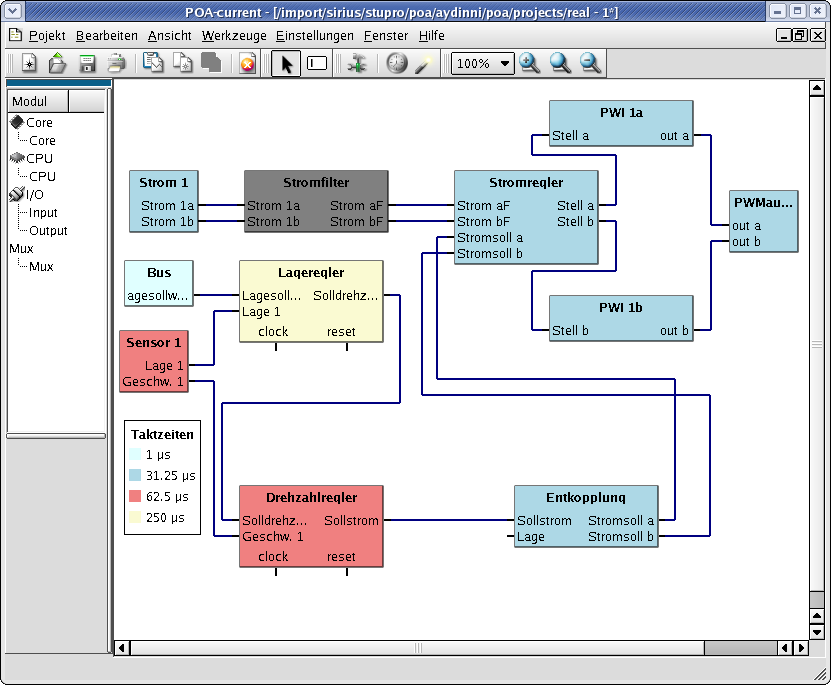
\includegraphics[width=10cm]{Mainwindow1}

\caption{Mainwindow}\label{test}

\end{center}

\end{figure}

Die Men"uleiste besteht aus den Men"us Project, Edit, View, Tools, Settings, Windows und Help.\par

Die hier Kurz beschriebenen Funktionen werden in den folgenden Abschnitten n"aher erkl"art.\par

\begin{itemize}
\item {\bf Project:}	New, Open, Save, Save as, Print, Recent, Exit\newline
Unter Project hat man die M"oglichkeit Projekte anzulegen, zu "offnen, abzuspeichern, auszudrucken und POA zu benden.
\item {\bf Edit:}	Cut, Copy, Paste\newline
Unter diesem Men"upunkt kann man die Aktionen Ausschneiden, Kopieren und Einf"ugen ausf"uhren.
\item {\bf View:}	Zoom in, Zoom normal, Zoom out\newline
Unter View ist es m"oglich den Inhalt im Arbeitsfenster anzuzoomen.
\item {\bf Tools:} 	Configuration, Route, Scheduling, Deploy Project\newline
Unter Tools k"onnen markierte Bl"ocke konfiguriert oder markierte Verbindungen geroutet werden. Au"serdem kann man hier im Untermen"u Scheduling den Ablauf f"ur die Bl"ocke grafisch darstellen und manipulieren. Das Untermen"u Deploy Project bietet die M"oglichkeit am Projekt ein Konsistenzcheck durchzuf"uhren.
\item {\bf Settings:}	Show Grid, Configure POA\newline
Unter Settings k"onnen Grundeinstellungen an POA vorgenommen werden.
\item {\bf Windows:} 	Tile, Tile Horizotal, Cascade\newline
Hier k"onnen, falls mehrere Projekte gleichzeitig ge"offnet sind, die Arbeitsfenster je nach Wunsch nebeneinander, "ubereinander oder kaskardiert angezeigt werden.
\item {\bf Help:} 	Contens, About\newline
Unter Help finden allgemeine Informationen "uber POA.\par
\end{itemize}

Die wichtigsten Aktionen k"onnen auch mit den Befehlsbuttons in der Symbolleiste oder im Kontextmen"u beim Markieren mit der rechten Maustaste ausgew"ahlt werden.

%\section{Dailogen}
%
%\subsubsection{POA Konfiguration Dailog}
%In diesem Konfigurationsdialog k"onnen alle m"oglichen Softwareeinstellungen vorgenommen %werden.
%\begin{figure}[htbp]
%\begin{center}
%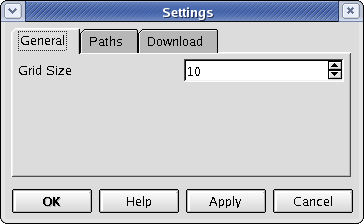
\includegraphics[width=10cm]{POAConfiguration1}
%\caption{POA Configuration}\label{test}
%\end{center}
%\end{figure}
%
%\subsubsection{Block Konfiguration Dailog}
%In diesem Konfigurationsdialog k"onnen die Bl"ocke (CPUs, Cores, Input-Block,
%Output-Block, Mux-Block) so konfiguriert werden, dass sie mit dem vorgegebenen
%CPLD-Design "ubereinstimmen.
%\begin{figure}[htbp]
%\begin{center}
%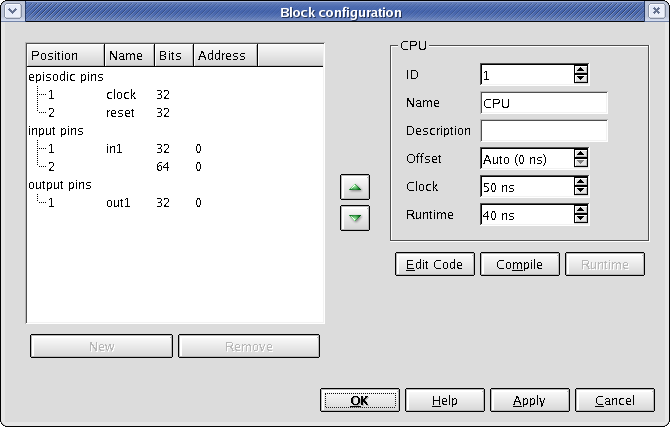
\includegraphics[width=10cm]{CPUConfiguration}
%\caption{Block Configuration}\label{test}
%\end{center}
%\end{figure}
%
%\subsubsection{Scheduling Dailog}
%In diesem Dialog werden Laufzeit, Takt und Offset der Bl"ocke visuell dargestellt. "Uber den %Offset der Bl"ocke kann eine Optimierung des CPLDs angestrebt werden.
%\begin{figure}[htbp]
%\begin{center}
%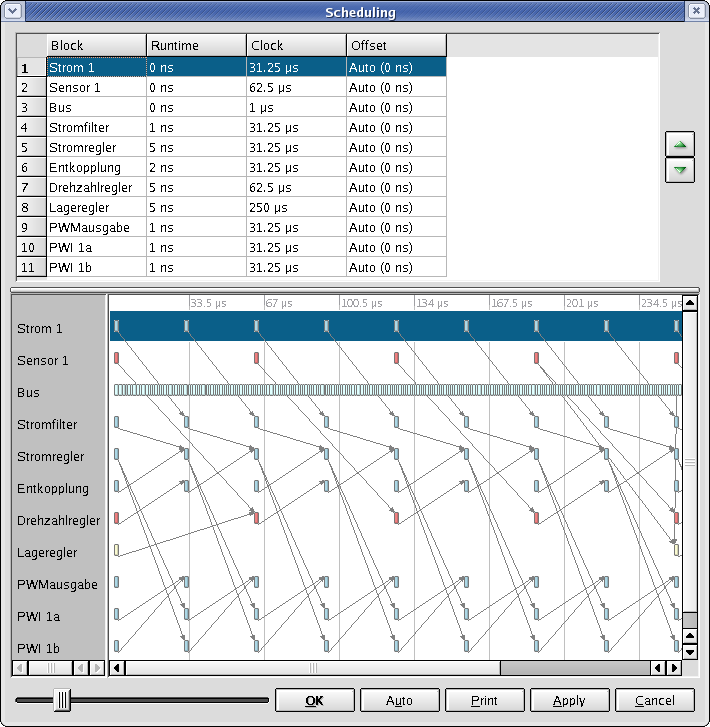
\includegraphics[width=10cm]{Scheduling1}
%\caption{Scheduling}\label{test}
%\end{center}
%\end{figure}
%
%\subsubsection{Wizard Dailog}


%%%%%%%%%%%%%%%%%%%%%%%%%%%%%%%%%%%%%%%%%%%%%%%%%%%%%%%%%%%%%%%%%%%%%%%%%%%%%
%%%%%%%%%%%%%%%%%%%%%%%%%%%%%%%%%%%%%%%%%%%%%%%%%%%%%%%%%%%%%%%%%%%%%%%%%%%%%

\chapter{Referenz}

\section{Beschreibung der Standard Tasten}
\begin{figure}[htbp]

\begin{center}

%%\includegraphics[width=10cm]{OK1}

\caption{Tasten}\label{test}

\end{center}

\end{figure}
Mit {\bf OK} werden die Einstellungen f"ur das Projekt gespeichert und der Dialog wird geschlossen.\par
Mit {\bf Apply} werden die Einstellungen "ubernommen.\par
Mit {\bf Cancel} werden die Einstellungen verworfen und der Dialog wird geschlossen.\par
Die Taste {\bf Help} ist in dieser Version von POA nicht belegt.


%%%%%%%%%%%%%%%%%%%%%%%%%%%%%%%%%%%%%%%%%%%%%%%%%%%%%%%%%%%%%%%%%%%%%%%%%%%%%
%%%%%%%%%%%%%%%%%%%%%%%%%%%%%%%%%%%%%%%%%%%%%%%%%%%%%%%%%%%%%%%%%%%%%%%%%%%%%
\section{POA konfigurieren}

\subsection{Raster einstellen}
\begin{figure}[htbp]

\begin{center}

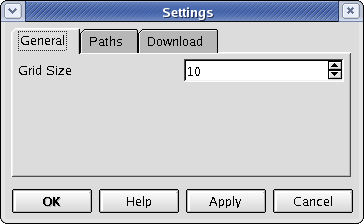
\includegraphics[width=10cm]{POAConfiguration1}

\caption{POA Konfiguration}\label{test}

\end{center}

\end{figure}
Die Bl"ocke und Verbindungen richten sich im Arbeitsfenster einem vorgegebenen Raster aus.\par

Zur Ver"anderung der Rastergr"o"se muss man im Untermen"u von {\bf Settings} den Eintrag {\bf Configure POA} ausw"ahlen. Im aufklappenden Dialog kann man unter dem Dateireiter {\bf General} die gew"unschte Rastergr"o"se eingeben.\par
Man kann das Raster anzeigen lassen oder ausblenden. Dazu w"ahlt man im Untermen"u von {\bf Settings} den Eintrag {\bf Show Grid} oder man dr"uckt die rechte Maustaste und w"ahlt {\bf Show Grid} im Kontextmen"u.


%%%%%%%%%%%%%%%%%%%%%%%%%%%%%%%%%%%%%%%%%%%%%%%%%%%%%%%%%%%%%%%%%%%%%%%%%%%%%
\subsection{Sprache einstellen}
POA unterst"utzt die Sprachen Deutsch und Englisch.\par
Zur Ver"anderung der Sprache muss man im Untermen"u von {\bf Settings} den Eintrag {\bf Configure POA} ausw"ahlen. Im aufklappenden Dialog kann man unter dem Dateireiter {\bf General} in der Auswahlbox {\bf Language} zwischen Englisch und Deutsch w"ahlen.\par

%%%%%%%%%%%%%%%%%%%%%%%%%%%%%%%%%%%%%%%%%%%%%%%%%%%%%%%%%%%%%%%%%%%%%%%%%%%%%
\subsection{Externe Programme einbinden}
POA bietet die M"oglichkeit externe Programme einzubinden und sie direkt und konfortabel aus POA heraus zu starten. Mit einem Editor kann der Quellcode f"ur die CPU in der Programmiersprache C  verfasst werden. Zum Kompilieren ben"otigt POA einen C-Compiler und f"ur das Herunterladen auf die CPLD wird ein Download Tool ben"otigt.\par
Zur Einbindung der externen Programme muss man im Untermen"u von {\bf Settings} den Eintrag {\bf Configure POA} w"ahlen. Im aufklappenden Dialog kann man unter dem Dateireiter {\bf Paths} die gew"unschten Programme einbinden.

\begin{figure}[htbp]

\begin{center}

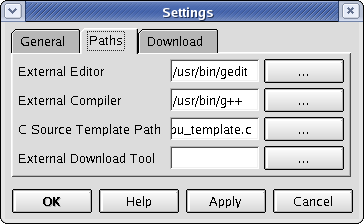
\includegraphics[width=10cm]{POAConfiguration2}

\caption{POA Konfiguration}\label{test}

\end{center}

\end{figure}

\subsubsection{Externen Editor einbinden}
Um einen Editor einzubinden, w"ahlt man unter dem Dateireiter {\bf Paths} das Textfeld neben {\bf External Editor} aus und gibt hier den korrekten Pfad des Editors ein. Alternativ dazu kann man auch mit dem Button neben dem Textfeld im Verzeichnisbaum nach dem gew"unschten Editor suchen.\par
\subsubsection{Externen Compiler einbinden}
Um einen Compiler einzubinden, w"ahlt man unter dem Dateireiter {\bf Paths} das Textfeld neben {\bf External Compiler} aus und gibt hier den korrekten Pfad des Compilers ein. Alternativ dazu kann man auch mit dem Button neben dem Textfeld im Verzeichnisbaum nach dem gew"unschten Compiler suchen.\par
\subsubsection{Externen Download Tool einbinden}
Um einen Download Tool einzubinden, w"ahlt man unter dem Dateireiter {\bf Paths} das Textfeld neben {\bf External Download Tool} aus und gibt hier den korrekten Pfad des Download Tool ein. Alternativ dazu kann man auch mit dem Button neben dem Textfeld im Verzeichnisbaum nach dem gew"unschten Download Tool suchen. \par
\newpage

%%%%%%%%%%%%%%%%%%%%%%%%%%%%%%%%%%%%%%%%%%%%%%%%%%%%%%%%%%%%%%%%%%%%%%%%%%%%%
\subsection{C Source Template Pfad angeben}
Mit dem C Source Template wird der Rahmencode f"ur den Quellcode der CPU vorgegeben.
Um einen C Source Template Pfad anzugeben, w"ahlt man unter dem Dateireiter {\bf Paths} das Textfeld neben {\bf C Source Template Path} aus und gibt hier den korrekten Pfad ein. Alternativ dazu kann man auch mit dem Button neben dem Textfeld im Verzeichnisbaum nach dem gew"unschten Pfad suchen. \par


%%%%%%%%%%%%%%%%%%%%%%%%%%%%%%%%%%%%%%%%%%%%%%%%%%%%%%%%%%%%%%%%%%%%%%%%%%%%%
\subsection{Download Einstellung}
\begin{figure}[htbp]

\begin{center}

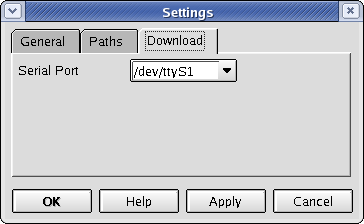
\includegraphics[width=10cm]{POAConfiguration3}

\caption{POA Konfiguration}\label{test}

\end{center}

\end{figure}
F"ur Downloadeinstellungen w"ahlt man den Dateireiter {\bf Download}. Hier kann man in der Auswahlbox den Seriellen Port, an dem das Board angeschlossen ist, einstellen.\par

\newpage
%%%%%%%%%%%%%%%%%%%%%%%%%%%%%%%%%%%%%%%%%%%%%%%%%%%%%%%%%%%%%%%%%%%%%%%%%%%%%
%%%%%%%%%%%%%%%%%%%%%%%%%%%%%%%%%%%%%%%%%%%%%%%%%%%%%%%%%%%%%%%%%%%%%%%%%%%%%
\section{Ein Projekt anlegen, "offnen, speichern}
\begin{figure}[htbp]

\begin{center}

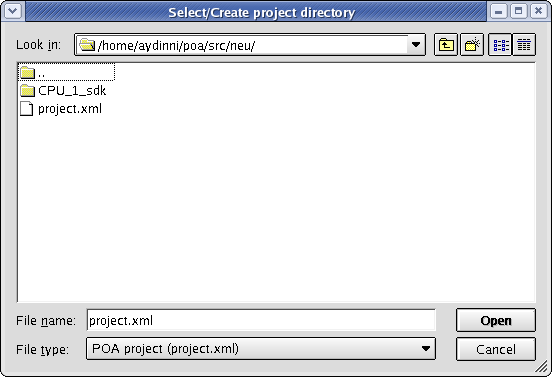
\includegraphics[width=10cm]{Directory}

\caption{Projekt Directory}\label{test}

\end{center}

\end{figure}

\subsection{Neues Projekt anlegen}
Durch anklicken des Men"us {\bf Project} in der Men"uleiste erscheint ein Untermen"u {\bf New}. Wenn dies ausgew"ahlt wird, wird ein Dailog ge"offnet, in dem man den Pfad f"ur das neue Projekt anlegen kann.\par

Ein neues Projekt kann auch durch einen Mausklick auf das Symbol {\bf New} in der Symbolleiste angelegt werden.
Wird ein neues Projekt angelegt, dann wird dadurch auch das Arbeitsfenster im Hauptfenster aktiviert.


%%%%%%%%%%%%%%%%%%%%%%%%%%%%%%%%%%%%%%%%%%%%%%%%%%%%%%%%%%%%%%%%%%%%%%%%%%%%%
\subsection{Bestehendes Projekt "offnen}
Im Untermen"u von {\bf Project} den Eintrag {\bf Open} oder in der Symbolleiste den {\bf Ordner} anklicken. Im nun aufklappendem Dialog kann man im Verzeichnisbaum das gew"unschte Projekt (project.xml-Datei) suchen und mit einem Doppelklick auf die Datei oder mit dem {\bf Open} Button "offen.
Im Arbeitsfenster erscheint nun das Projekt mit den Funktionsbl"ocken (CPUs, Cores,..) und den Verbindungen, d.h. dem Vernetzungsplan.\par


%%%%%%%%%%%%%%%%%%%%%%%%%%%%%%%%%%%%%%%%%%%%%%%%%%%%%%%%%%%%%%%%%%%%%%%%%%%%%
\subsection{Projekt speichern}
Im Untermen"u von {\bf Project} den Eintrag {\bf Save} oder in der Symbolleiste die {\bf Diskette} anklicken. Dabei wird das Projekt automatisch in das urspr"ungliche Verzeichnis gespeichert.\par
Mit dem Eintrag {\bf Save as} kann das Projekt in ein anderes Verzeichnis gespeichert werden. Dabei wird ein Dialog ge"offnet, in den man das Verzeichnis angeben kann.\par


%%%%%%%%%%%%%%%%%%%%%%%%%%%%%%%%%%%%%%%%%%%%%%%%%%%%%%%%%%%%%%%%%%%%%%%%%%%%%
%%%%%%%%%%%%%%%%%%%%%%%%%%%%%%%%%%%%%%%%%%%%%%%%%%%%%%%%%%%%%%%%%%%%%%%%%%%%%
\section{Layout drucken}
\begin{figure}[htbp]

\begin{center}

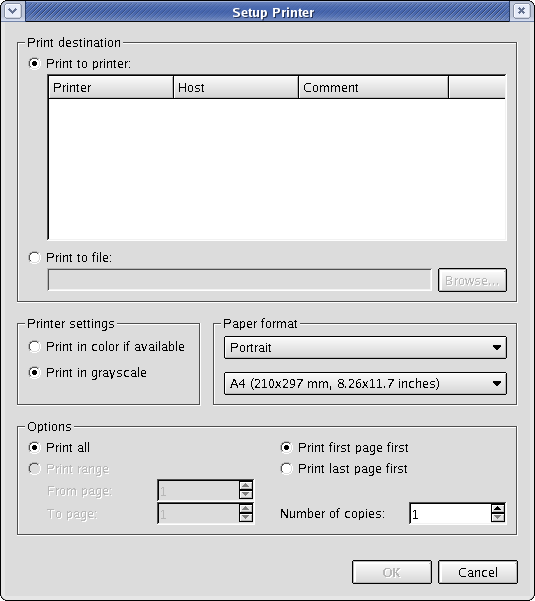
\includegraphics[width=10cm]{Printer}

\caption{Setup Printer}\label{test}

\end{center}

\end{figure}
POA bietet die M"oglichkeit das entworfene Layout und die grafische Darstellung des Scheduling zu drucken oder als druckbare Datei zu speichern.
Im Untermen"u {\bf Project} den Eintrag {\bf Print} oder in der Symbolleiste den {\bf Drucker} w"ahlen. Im nun aufklappendem Dialog kann man die gew"unschten Druckeinstellungen vornehmen und den Druckauftrag an den ausgew"ahlten Drucker mit der Best"atigung durch {\bf OK} schicken.\par
Mit {\bf Cancel} werden die Einstellungen verworfen.\par






%%%%%%%%%%%%%%%%%%%%%%%%%%%%%%%%%%%%%%%%%%%%%%%%%%%%%%%%%%%%%%%%%%%%%%%%%%%%%
%%%%%%%%%%%%%%%%%%%%%%%%%%%%%%%%%%%%%%%%%%%%%%%%%%%%%%%%%%%%%%%%%%%%%%%%%%%%%
\section{Bl"ocke}

\subsection{Bl"ocke erzeugen}
Bl"ocke, wie CPUs, Cores etc. k"onnen per Drag'n Drop aus der Blockbibliothek in das Arbeitsfenster gezogen werden und dadurch erzeugt werden. Wenn man ein Block ins Arbeitsfenster gezogen hat und die Maustaste wieder losläst, wird automatisch das Konfigurationsfenster f"ur den Block ge"offnet. Hier hat man die M"oglichkeit verschiedene Einstellungen vornehmen.

%%%%%%%%%%%%%%%%%%%%%%%%%%%%%%%%%%%%%%%%%%%%%%%%%%%%%%%%%%%%%%%%%%%%%%%%%%%%%
\subsection{Bl"ockkonfiguration allgemein}
Beim Erzeugen eines Blocks wird ein Kofigurationsdialog automatisch ge"offnet. Hier hat man je nach Block verschiedene Konfigurationsm"oglichkeiten. Der Konfigurationsdialog kann auch sp"ater ge"offnet werden. Dazu w"ahlt man den zu konfigurierenden Block mit der rechten Maustaste aus und w"ahlt im Kontextmen"u den Eintrag {\bf Configuration}, oder man f"uhrt ein Doppelklick mit der linken Maustaste auf den Block aus.\par
Alternativ dazu kann man f"ur den ausgew"ahlten Block die Funktion auch "uber die Men"uleiste oder Symbolleiste ausf"uhren. \par

\begin{figure}[htbp]

\begin{center}

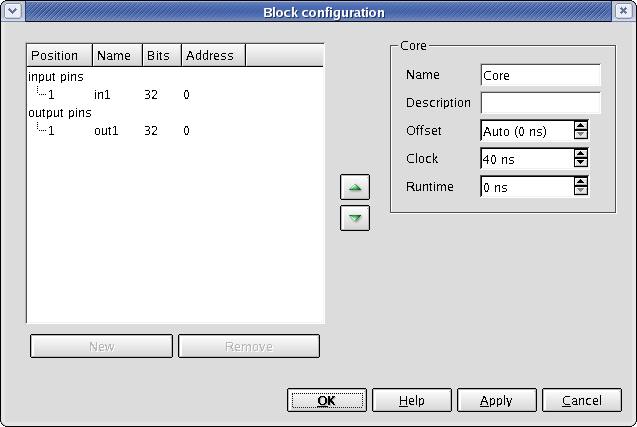
\includegraphics[width=10cm]{CoreBlockConfiguration}

\caption{Block Konfiguration}\label{test}

\end{center}

\end{figure}

D
\subsubsection{Blockname "andern}
Zur eindeutigen Identifizierung der Bl"ocke ist es von Vorteil der Bl"ocken einen aussagekräftigen Namen zu geben.\par
Im Textfeld {\bf Name} kann man den neuen Namen des Blocks eingeben.
\subsubsection{Block beschreiben}
Im Textfeld {\bf Description} kann man Beschreibungen oder Komentare zum Block eingeben.\par
Die Blockbeschreibung hat den Vorteil, dass man sp"ater auch noch leicht nachvollziehen kann, wof"ur dieser Block gut ist.\par
Diese Option ist f"ur {\bf Multiplexer} nicht verf"ugbar.
\subsubsection{Neue Pins erzeugen}
In der Pinbibliothek k"onnen blockabh"angig drei verschiedene Arten von Pins ("'Episodic Pin"', "'Input Pin"' und "'Output Pin"') verwaltet werden. Je nach Pinart w"ahlt man in der Bibliothek die entsprechende Kategorie. Dabei wird der {\bf New} Button aktiviert. Mit einem Kick auf den aktivierten {\bf New} Button wird ein neuer Pin erzeugt. \par
\subsubsection{Pins l"oschen}
Dazu w"ahlt man in der Pinbibliothek den zu l"oschende Pin aus. Der {\bf Remove} Button wird nun aktiviert. Mit einem Mausklick auf den {\bf Remove} Button wird der Pin gel"oscht. Wenn an diesem Pin eine Verbindung angedockt war, wird diese Verbindung automatisch gel"oscht.
\subsubsection{"Anderungen an Pins vornehmen}
Dazu w"ahlt man in der Pinbibliothek den zu "andernde Pin aus.\par
Unter der Spalte {\bf Name} kann man dem Pin einen Namen geben oder einen vorhandenen Namen "andern.\par
Unter der Spalte {\bf Bits} kann die Anzahl der Bits f"ur ein Pin "andern werden.\par
Unter der Spalte {\bf Address} kann eine Adressierung f"ur die Input-Pins und Output-Pins vornehmen werden.\par
\subsubsection{Offset eingeben}
Um das Offset an dem Block einzugeben, kann man entweder direkt mit der Maus ins Textfeld {\bf Offset} klicken und die Offsetzeit in Nanosekunden eingeben oder man benutzt die Pfeiltasten neben dem Textfeld.\par
Diese Option ist f"ur {\bf Multiplexer} nicht verf"ugbar.
\subsubsection{Takt eingeben}
Um die Taktrate des Blocks einzugeben, kann man entweder direkt mit der Maus ins Textfeld {\bf Clock} klicken und die Taktfrequenz in Nanosekunden eingeben oder man benutzt die Pfeiltasten neben dem Textfeld.\par
Diese Option ist f"ur {\bf Multiplexer} nicht verf"ugbar.
\subsubsection{Laufzeit eingeben}
Um die Laufzeit des Blocks einzugeben, kann man entweder direkt mit der Maus ins Textfeld{\bf Runtime} klicken und die Laufzeit in Nanosekunden eingeben oder man benutzt die Pfeiltasten neben dem Textfeld.\par
Diese Option ist f"ur {\bf Multiplexer} und {\bf Inputbl"ocke} nicht verf"ugbar.


%%%%%%%%%%%%%%%%%%%%%%%%%%%%%%%%%%%%%%%%%%%%%%%%%%%%%%%%%%%%%%%%%%%%%%%%%%%%%
\subsection{I/O Block konfigurieren}
Siehe Kapitel {\bf Blockkonfiguration allgemein}.

%\begin{figure}[htbp]
%\begin{center}
%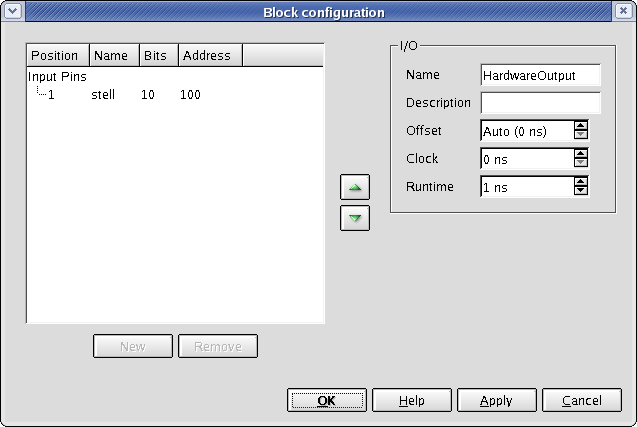
\includegraphics[width=10cm]{OutputBlockConfiguration}
%\caption{I/O Block Configuration}\label{test}
%\end{center}
%\end{figure}


%%%%%%%%%%%%%%%%%%%%%%%%%%%%%%%%%%%%%%%%%%%%%%%%%%%%%%%%%%%%%%%%%%%%%%%%%%%%%
\subsection{Core konfigurieren}
Siehe Kapitel {\bf Blockkonfiguration allgemein}.


%%%%%%%%%%%%%%%%%%%%%%%%%%%%%%%%%%%%%%%%%%%%%%%%%%%%%%%%%%%%%%%%%%%%%%%%%%%%%
\subsection{CPU konfigurieren}
\begin{figure}[htbp]

\begin{center}

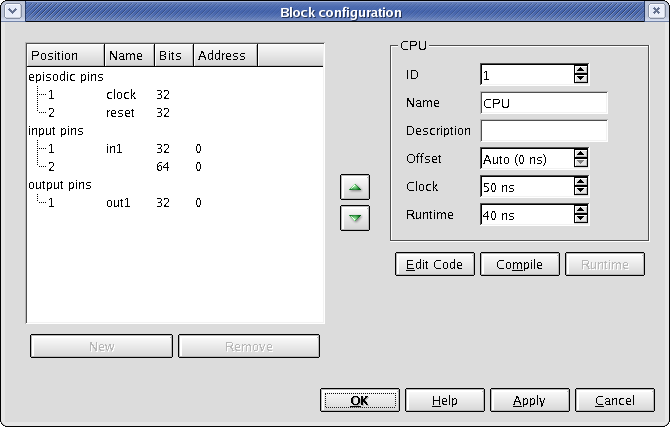
\includegraphics[width=10cm]{CPUConfiguration}

\caption{CPU Konfiguration}\label{test}

\end{center}

\end{figure}
\subsubsection{ID eingeben}
Jeder CPU muss eine ID (d.h. eine Nummer von 0 - 99) vergeben werden, dazu kann man entweder direkt mit der Maus ins Textfeld {\bf ID} klicken und die Nummer eingeben oder man benutzt die Pfeiltasten neben dem Textfeld.

\subsubsection{Die CPU-Programmcode schreiben}
Zum Schreiben von CPU-Programmcode wird ein externer Editor aufgerufen, wenn im Konfigurationsdialog der Button {\bf Edit Code} gedr"uckt wird. Beim "Offnen des des Editors wird automatisch ein C-Source Template geladen, der einen generierten Rahmencode f"ur die CPU in der Programmiersprache C vorgibt. Im Editor kann dann der restliche Quellcode f"ur die CPU niederschreiben und abspeichern.

\subsubsection{CPU-Programmcode kompilieren}
Zum Kompilieren des erzeugten CPU-Programmcodes wird ein externer Compiler gestartet, wenn im Konfigurationsdialog der Button {\bf Compile} gedr"uckt wird. Der Compiler kompiliert den CPU-Programmcode und gibt im {\bf POA Terminal} eine entsprechende Meldung aus.

\begin{figure}[htbp]

\begin{center}

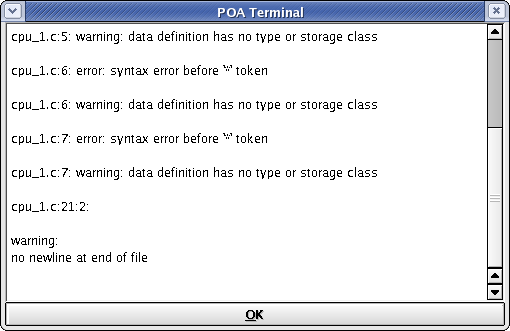
\includegraphics[width=10cm]{Terminal}

\caption{POA Terminal}\label{test}

\end{center}

\end{figure}
\newpage



%%%%%%%%%%%%%%%%%%%%%%%%%%%%%%%%%%%%%%%%%%%%%%%%%%%%%%%%%%%%%%%%%%%%%%%%%%%%%
\subsection{Multiplexer konfigurieren}
\begin{figure}[htbp]

\begin{center}

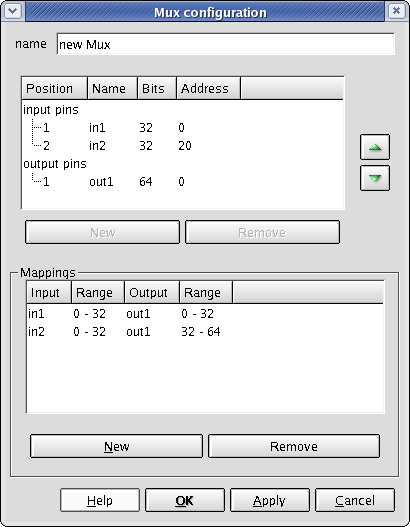
\includegraphics[width=10cm]{MuxConfiguration}

\caption{Multiplexer Konfiguration}\label{test}

\end{center}

\end{figure}

Multiplexer dienen dazu mehrere Eingangssignale auf ein Ausgangssignal zu reduzieren.

%%%%%%%%%%%%%%%%%%%%%%%%%%%%%%%%%%%%%%%%%%%%%%%%%%%%%%%%%%%%%%%%%%%%%%%%%%%%%
\subsection{Bl"ocke in Arbeitsfenster verschieben}
W"ahlen Sie das Block mit der linken Maustaste aus, lassen Sie Taste gedr"uckt und verschieben das Block in Arbeitsfenster bis Sie die gew"unschte Position haben. Dabei werden die Verbindungen, die an diesem Block h"angen automatisch mitgeroutet.


%%%%%%%%%%%%%%%%%%%%%%%%%%%%%%%%%%%%%%%%%%%%%%%%%%%%%%%%%%%%%%%%%%%%%%%%%%%%%
\subsection{Block kopieren und einf"ugen}
Wenn Sie mehrere identische Bl"ocke f"ur Ihr Layout ben"otigen eignet sich dazu die "'copy and paste"' Funktion. Hierzu w"ahlen Sie das Block mit der rechten Maustaste aus. Im KontextMen"u w"ahlen Sie den Eintrag {\bf Copy}. Wenn Sie nun mit der linken Maustaste auf ein freies Feld in Arbeitsfenster
klicken, k"onnen Sie im KontextMen"u den Eintrag {\bf Paste} w"ahlen, um eine Kopie des ausgew"ahlten Blocks zu erzeugen.
Die Kopie wird automatisch im linken oberen Rand des Arbeitsfensters positioniert.\par
Altenativ k"onnen Sie diese Aktion auch "uber die Men"uleiste bzw. Symbolleiste ausf"uhren.


%%%%%%%%%%%%%%%%%%%%%%%%%%%%%%%%%%%%%%%%%%%%%%%%%%%%%%%%%%%%%%%%%%%%%%%%%%%%%
\subsection{Block ausschneiden und einf"ugen}
Hierbei gehen Sie wie zuvor im Abschnitt "'Bl"ocke kopieren und einf"ugen"' vor, mit der Aunahme, dass Sie statt der Aktion {\bf Copy} die Aktion {\bf Cut} w"ahlen. \par
Wenn ein Block ausgeschnitten wird, werden alle Verbindungen mit diesem Block unwiderruflich gel"oscht.


%%%%%%%%%%%%%%%%%%%%%%%%%%%%%%%%%%%%%%%%%%%%%%%%%%%%%%%%%%%%%%%%%%%%%%%%%%%%%
\subsection{Block l"oschen}
W"ahlen Sie das zul"oschende Block mit der rechten Maustaste aus. Im KontextMen"u w"ahlen Sie den Eintrag {\bf Remove} und das Block wird unwiderruflich gel"oscht.\par
Altenativ k"onnen Sie f"ur das ausgew"ahlte Block diese Aktion auch "uber die Men"uleiste bzw. Symbolleiste ausf"uhren.\par
Wenn ein Block gel"oscht wird, werden alle Verbindungen mit diesem Block auch unwiderruflich gel"oscht.


%%%%%%%%%%%%%%%%%%%%%%%%%%%%%%%%%%%%%%%%%%%%%%%%%%%%%%%%%%%%%%%%%%%%%%%%%%%%%
%%%%%%%%%%%%%%%%%%%%%%%%%%%%%%%%%%%%%%%%%%%%%%%%%%%%%%%%%%%%%%%%%%%%%%%%%%%%%
\section{Verbindungen}
\subsection{Verbindung routen}

\subsubsection{Bl"ocke miteinander verbinden}
Hierzu klicken Sie mit der linken Maustaste auf den Pin des Blocks und lassen Sie die Maustaste gedr"uckt. Die Verbindungsm"oglichkeiten werden nun gr"un angezeigt. Sie k"onnen jetzt mit dem Mauszeiger an ein Pin eines anderen Blocks andocken. Dabei muss die linke Maustaste immer gedr"uckt bleiben. Nachdem Sie am Pin angedockt haben, k"onnen Sie die Maustaste wieder los lassen und die Verbindung (Connector) wird nun automatisch gezogen. Verbindungen k"onnen nur durch senkrechte oder waagrechte Linien dargestellt werden.

\subsubsection{Verbindung automatisch routen}
Es gibt zwei verschiedene M"oglichkeiten des automatischen Routens:
\begin{itemize}
\item der Default Router ist der Standartrouter der automatisch beim erzeugen einer Verbindung benutzt wird.
\item der Smart Router kann nach Erzeugung einer Verbindung eingesetzt werden, um eventuell "uberlappende Verbindungen "uberlappungsfrei darzustellen.
\end{itemize}
Wenn Sie eine Verbindung automatisch routen m"ochten, w"ahlen Sie die Verbindung mit rechten Maustaste aus,w"ahlen Sie im KontextMen"u den Eintrag {\bf Routen} und klicken Sie unter {\bf Routen} auf den gew"unschte Router ({\bf Default Router} oder {\bf Smart Router}).

\subsubsection{Verbindung manuell routen}
Zum manuellen Routen m"ussen Sie die Verbindung mit der linken Maustaste ausw"ahlen. Nun k"onnen Sie mit gedr"uckter Maustaste einen Verbindungsabschnitt entweder horizontal oder vertikal verschieben. Das hei"st ein horizontaler Verbindungsabschnitt kann nur vertikal verschoben werden und ein vertikaler Verbindungsabschnitt nur horizontal. Beim Verschieben der einzelnen Abschnitte werden die anh"angenden Linien automatisch nachgezogen, sodass eine Verbindung immer bestehen bleibt.

%%%%%%%%%%%%%%%%%%%%%%%%%%%%%%%%%%%%%%%%%%%%%%%%%%%%%%%%%%%%%%%%%%%%%%%%%%%%%
\subsection{Verbindung l"oschen}
W"ahlen Sie die zul"oschende Verbindung mit der rechten Maustaste aus. Im KontextMen"u w"ahlen Sie nun den Eintrag {\bf Remove} und die Verbindung wird unwiderruflich gel"oscht.
Alternativ k"onnen Sie die zul"oschende Verbindung mit der linken Maustaste ausw"ahlen und danach das Symbol {\bf l"oschen} in der Symbolleiste oder die {\bf Enfernen} Taste dr"ucken.


\section{Scheduling}
\section{Deploy Project}
\section{Allgemein}
\subsection{Farbgebung}
\subsection{Beschriftung des Layouts}
\subsection{Zoomen}
\end{document}
